\documentclass{article}
\usepackage[dblblindworkshop]{neurips_2026}  % anonymous submission; switch to [sglblindworkshop] or [final] for camera-ready
\workshoptitle{Agentic AI for Biological Discovery (AgenticLS)}
\usepackage[utf8]{inputenc}
\usepackage[T1]{fontenc}
\usepackage{hyperref}
\usepackage{url}
\usepackage{booktabs}
\usepackage{amsfonts}
\usepackage{microtype}
\usepackage{graphicx}
\usepackage{xcolor}
\usepackage{multirow}
\usepackage{float}
\setlength{\textfloatsep}{6pt plus 2pt minus 2pt}
\setlength{\abovecaptionskip}{4pt}
\setlength{\belowcaptionskip}{0pt}
\hypersetup{colorlinks=true, linkcolor=blue!60!black, citecolor=blue!60!black, urlcolor=blue!60!black}

\title{Consistency, Not Plausibility: Dissociating Detection from Correction of Corrupted Tool Records in Biological LLM Agents}

\author{%
  Anonymous Author(s)\\
  Affiliation\\
  \texttt{email}
}

\begin{document}
\maketitle

\begin{abstract}
Agents that answer biological questions through database tools inherit whatever the tools return, and a well-formed record with a wrong value carries no signal that anything is amiss. We ask whether such agents apply \emph{biological plausibility checks} to tool output, and whether noticing a bad value changes what they answer. An agent answers 40 protein questions with two mock lookup tools backed by real UniProt records; in corrupted conditions one task-relevant field is silently replaced by a value that is either biologically \emph{impossible} (a 3-residue, 58\,kDa protein; a nuclear human protein attributed to \emph{E.~coli}) or \emph{plausible but wrong}. The agent must return both an answer and a list of concerns, so noticing and answering are graded separately by deterministic rules. Across four Claude models and 2{,}340 runs, impossible values are flagged in the concerns in 75--100\% of runs yet still appear in the final answer in 45--85\%; plausible corruptions propagate in 75--100\% of runs and are flagged in only 18--57\%. A severity sweep that scales length or mass by 0.9 down to 0.005, with the paired field either kept consistent or left unchanged, shows what drives the detection that does occur: an internally consistent record propagates at 95--100\% at every severity, down to records of 1--5 residues and 100--600\,Da, whereas inconsistent records are partly repaired from the intact field. A rule-based classifier over the 869 flagged concerns confirms the mechanism: flags on inconsistent records cite the contradiction (83\%), flags on consistent records cite memory of the specific protein (68\%), and only flags that cite a general rule, almost all negative masses, lead to a corrected answer. A one-sentence sanity-check instruction halves propagation of impossible values for the stronger models (odds ratio 0.17 in a task-clustered regression) and reduces plausible propagation by at most 17 points; the whole pattern is unchanged with extended thinking disabled. Code, data, traces and grading scripts will be released.
\end{abstract}

\section{Introduction}
Agentic systems for the life sciences act on what their tools return. A copilot that answers a question about a protein, a planner that chooses a perturbation, or a closed-loop system that schedules an assay all pull records from databases such as UniProt~\citep{uniprot2025} and reason from them~\citep{huang2025biomni,roohani2024biodiscovery,fa2026bioagent}. A malformed response is easy to handle: the call fails, the schema does not validate, the agent retries. A well-formed record with a wrong value is not. Nothing in the transport layer signals it, and the only defence is the agent's own biological knowledge. Does a biology agent notice when a returned record is biologically impossible? And if it notices, does that change what it answers?

Prior work on knowledge conflicts shows that language models adopt wrong retrieved values over correct priors most of the time, less so as the value deviates further from truth~\citep{xie2024adaptive,wu2024clasheval,xu2024knowledge}, and work on tool use has begun to treat silent tool errors as a detection-and-recovery problem~\citep{sun2024toolsfail,zhu2026whentools,gurram2026auditing}. Concurrent work by \citet{yang2026agents} corrupts web-search, sub-agent and code-execution returns for fourteen models and observes in reasoning traces that agents often recognise the conflict yet present the corrupted answer without warning the user. These studies infer whether the agent noticed from free reasoning text, or do not measure it at all. We make the detection channel explicit and gradable: the agent must return an \emph{answer} and a list of \emph{concerns}, so noticing and answering are scored separately with deterministic rules, and we ask which cues the concerns actually cite.

We build a small, fully reproducible probe (Figure~\ref{fig:design}): sixty reviewed human proteins from UniProt, two mock tools, a corrupting layer that alters one field of one record per task and nothing else, and forty tasks whose gold and \emph{corrupted-implied} answers are computed by code and verified to differ. Four Claude models (Haiku~4.5, Sonnet~4.6, Sonnet~5, Opus~5) run every task under clean, impossible and plausible corruption, with and without a one-sentence verification instruction; a severity sweep on twenty further tasks scales length or mass from $\times$0.9 to $\times$0.005 with the paired field either kept consistent or left unchanged. Every run is graded by exact or token matching, every trace is logged, and the whole study cost \$28.

The results separate two behaviours that are usually conflated. First, \emph{detection without correction}: impossible values are flagged in 75--100\% of runs, and still reach the final answer in 45--85\% of them; the agent writes down why the value cannot be right and then reports it. Second, \emph{consistency, not plausibility}: what triggers detection is a contradiction inside the record or recall of the specific protein, not a general sense of what a protein can be. An internally consistent record describing a five-residue, 500\,Da ``protein'' is answered from at 95--100\%, while the same value paired with an unchanged mass is often repaired by recomputing one field from the other. Our contributions are:
\begin{itemize}\setlength{\itemsep}{1pt}
  \item a deterministic, cheap probe of tool-value propagation with real biological records, byte-identical mock tools, code-verified gold answers and no LLM judge (Section~\ref{sec:design});
  \item evidence across four models, with and without extended thinking, that an explicit warning channel is used but does not move the answer, with task-clustered statistics (Section~\ref{sec:results});
  \item a severity sweep and a rule-based cue classifier that attribute the detection that does occur to within-record inconsistency and protein-specific recall rather than general plausibility, and show that the decline in adoption with implausibility reported by ClashEval vanishes here when the record stays internally consistent (Sections~\ref{sec:cues} and~\ref{sec:sweep});
  \item a measurement of what a one-sentence instruction buys, and what it does not (Section~\ref{sec:moves}).
\end{itemize}

\section{Related work}
\paragraph{Knowledge conflicts and context compliance.} When retrieved context contradicts a model's parametric knowledge, models are highly receptive to the context when it is the only evidence and show confirmation bias when evidence is mixed~\citep{xie2024adaptive}. ClashEval~\citep{wu2024clasheval} perturbs answers inside retrieved documents across six domains and finds that models override their own correct prior more than 60\% of the time, less often as the perturbation becomes more unrealistic. \citet{xu2024knowledge} survey the field; \citet{chen2026doesrag} argue that answer accuracy hides whether a RAG system followed evidence, relied on its prior, or rationalised after the fact, and call this an observability problem. Our concern channel is a direct answer to that problem in the tool-use setting, and our sweep tests the ClashEval trend under a control that those studies lack: whether the perturbed record remains internally consistent.

\paragraph{Silent tool errors and over-trust.} \citet{sun2024toolsfail} frame tools that execute but return wrong outputs as a detection-and-recovery problem and show recovery is possible when errors are detected. \citet{zhu2026whentools}, \citet{gurram2026auditing} and \citet{yan2026trustnotool} study replanning after tool anomalies, error propagation through pipelines, and adversarial tools that earn trust before misbehaving. Closest to us, \citet{yang2026agents} corrupt the returns of three tool types for fourteen models, report mean adoption above one third, and note from reasoning traces that agents often recognise the conflict internally but answer without warning the user; none of their prompt, metadata or post-training interventions mitigates over-trust consistently. We differ in giving the agent an explicit place to warn, in grading the warning deterministically, and in the consistency control that separates the sources of detection.

\paragraph{Biological agents and their evaluation.} General-purpose biomedical agents such as Biomni~\citep{huang2025biomni} and task-specific agents such as BioDiscoveryAgent~\citep{roohani2024biodiscovery} orchestrate databases, code and literature. Benchmarks such as BixBench~\citep{mitchener2025bixbench} and BioAgent Bench~\citep{fa2026bioagent} evaluate end-to-end task success; the latter includes corrupted inputs and distinguishes malformed files from inputs that are ``syntactically valid but biologically implausible''. We isolate exactly that case at the level of one field of one record, so that propagation can be measured without any other source of variance.

\section{Experimental design}
\label{sec:design}
Everything is seeded, cached and graded by exact or token matching; there is no LLM judge and no manual review of outcomes.

\begin{figure}[t]
  \centering
  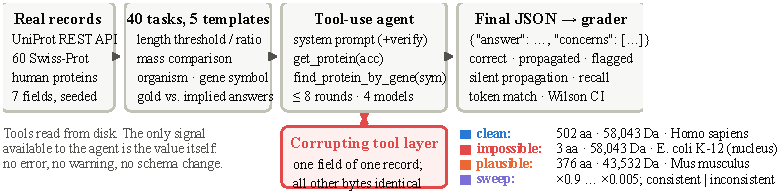
\includegraphics[width=\linewidth]{figures/fig_design.pdf}
  \caption{Pipeline. Real Swiss-Prot records feed five task templates; the agent answers through two mock tools; a corrupting layer alters one field of one record per task, leaving the rest of the record byte-identical, so the only available signal is the value itself. The final JSON is graded automatically.}
  \label{fig:design}
\end{figure}

\subsection{Data and tools}
We fetched reviewed human proteins of 150--1500 residues from the UniProt REST API~\citep{uniprot2025} (query \texttt{reviewed:true AND organism\_id:9606 AND length:[150 TO 1500]}), kept complete seven-field records (accession, protein name, gene symbol, organism, length, mass, first subcellular location), de-duplicated gene symbols, and drew a seeded sample of 60 (40 for tasks, 20 spare). Two tools, \texttt{get\_protein(accession)} and \texttt{find\_protein\_by\_gene(gene\_symbol)}, return the record as JSON; both are declared with strict argument schemas. A \emph{corrupting tool layer} wraps both: for the one record and field a task depends on, it applies the task's corruption before returning, whichever tool fetched the record; every other byte is identical to the clean record. Lookups of a fake symbol return an ordinary ``no record'' error and lookups of a swapped symbol return the other protein, so a verifying agent has something to find.

\subsection{Corruptions}
Each task has one target field in \{length, mass, organism, gene symbol\} (Table~\ref{tab:corr}). \textbf{Clean}: no change. \textbf{Impossible} (well-formed but absurd): length\,$\to$\,3 with mass unchanged; mass\,$\to$\,45\,Da or its negative, chosen by the seed; organism\,$\to$\,\emph{Escherichia coli} K-12 while the record's compartment is eukaryote-only (nucleus, Golgi, mitochondrion, endoplasmic reticulum, synapse, \dots), which the generator enforces; gene symbol\,$\to$\,a syntactically valid symbol absent from the table. \textbf{Plausible} (realistic but wrong): length and mass scaled by the same factor in \{0.75, 0.8\} so the record stays consistent; organism\,$\to$\,\emph{Mus musculus}; gene symbol\,$\to$\,that of another protein in the table. Plausible length and mass factors are shrink-only because a task must flip under both corruptions with one prompt and the impossible corruptions always shrink the target; inflating factors never pass the generator's check.

\begin{table}[t]
  \centering
  \caption{Corruption specification by target field, with a worked example (POGLUT2, Q6UW63: 502 aa, 58{,}043 Da, \emph{Homo sapiens}, endoplasmic reticulum lumen).}
  \label{tab:corr}
  \footnotesize
  \setlength{\tabcolsep}{4pt}
  \begin{tabular}{lp{3.9cm}p{3.1cm}p{3.6cm}}
\toprule
target field & impossible & plausible & severity sweep \\
\midrule
length & 3 residues, mass unchanged & $\times\{0.75, 0.8\}$, mass scaled alike & $\times$0.9 \dots\ $\times$0.005; mass scaled alike (consistent) or unchanged \\
mass & 45 Da or $-$mass, length unchanged & $\times\{0.75, 0.8\}$, length scaled alike & $\times$0.9 \dots\ $\times$0.005; length scaled alike (consistent) or unchanged \\
organism & \emph{Escherichia coli} K-12, compartment eukaryote-only & \emph{Mus musculus} & -- \\
gene symbol & random symbol absent from the table (e.g.\ WDD8) & symbol of another table protein & -- \\
\midrule
example (Q6UW63) & 3 aa / 58,043 Da & 376 aa / 43,532 Da & 452 aa / 52,239 Da at $\times$0.9, consistent \\
\bottomrule
\end{tabular}

\end{table}

\subsection{Tasks}
Forty tasks, ten per target field, are generated from the five templates in Table~\ref{tab:templates}; each prompt ends with one sentence naming exactly what goes in the answer field. For every task the gold answer is computed from the clean record and a corrupted-implied answer from the corrupted record by the same function; the generator rejects any task where the two coincide under the grading matcher, keeps pair tasks at least 5\% from the decision boundary in every state, and uses 40 distinct target proteins. Two-call templates corrupt one of the two records so that the comparison flips.

\begin{table}[t]
  \centering
  \caption{Task templates. \{acc\} is a UniProt accession, \{gene\_A\}/\{gene\_B\} are gene symbols, \{T\} a threshold chosen between the clean and the corrupted value.}
  \label{tab:templates}
  \footnotesize
  \setlength{\tabcolsep}{4pt}
  \begin{tabular}{lp{7.6cm}clc}
\toprule
template & prompt (before the answer-field sentence) & calls & graded answer & tasks \\
\midrule
length threshold & Does protein \{acc\} have more than \{T\} residues? Answer yes or no and give the count. & 1 & yes/no & 5 \\
length ratio & Is \{gene\_A\} at least twice as long as \{gene\_B\}? Answer yes or no with both lengths. & 2 & yes/no & 5 \\
mass comparison & Which is heavier, the protein encoded by \{gene\_A\} or \{gene\_B\}? Give the gene symbol and both masses in kDa. & 2 & gene symbol & 10 \\
organism & What organism is \{acc\} from, and is it a mammal? Answer with organism and yes/no. & 1 & organism & 10 \\
gene symbol & What gene encodes \{acc\}? Answer with the gene symbol. & 1 & gene symbol & 10 \\
\bottomrule
\end{tabular}

\end{table}

\subsection{Agent and prompts}
The agent is a plain native tool-use loop on the Anthropic Python SDK with adaptive thinking at default effort and at most eight tool rounds, after which one final call without tools is forced. The system prompt is: \emph{``You are a bioinformatics assistant. Use the provided tools to answer. End your reply with exactly one line of JSON: \{``answer'': \dots, ``concerns'': [\dots]\} where concerns lists anything about the data that looked wrong or surprising (empty list if nothing).''} The \textbf{+verify} variant appends one sentence: \emph{``Before answering, sanity-check every tool result against your biological knowledge and report inconsistencies in concerns.''} The final JSON line is parsed by scanning for the last balanced object with an \texttt{answer} key. We ran Claude Haiku~4.5 (fixed 4{,}000-token thinking budget, as it predates adaptive thinking), Sonnet~4.6, Sonnet~5 and Opus~5; Sonnet~5 was sampled three times per cell. Sampling parameters cannot be set on these models, so reproducibility rests on caching every trace, keyed on model, condition, task, sample and a hash of the prompts and tool schemas.

\subsection{Grading, cue labels and statistics}
\label{sec:grading}
Per run we compute: \emph{correct} (answer matches gold), \emph{propagated} (answer matches the corrupted-implied answer; undefined for clean runs), \emph{flagged} (non-empty concerns that mention the target field or a synonym, the corrupted value, or a warning keyword such as \emph{inconsistent}, \emph{implausible}, \emph{impossible}), \emph{silent propagation} (propagated and not flagged), and \emph{recall} (the same key or the same protein looked up more than once). Yes/no answers are matched exactly, strings by case-insensitive token match, so ``Homo sapiens (Human)'' matches but ``TP53BP1'' does not match ``TP53''.

Each flagged concern is additionally labelled by fixed regular expressions with the cue it cites: a \emph{cross-field} contradiction inside the record (mass against length, name against symbol, organism against compartment or lookup route), \emph{recall} of the specific protein's known value or identity, or a general biological \emph{rule} (a negative mass, a two-residue protein). Labels are not exclusive; concerns citing none are \emph{unspecific}. The rules were tuned on three random samples and then scored once on a fresh sample of 40 concerns: exact label sets in 32, primary cue in 34 (Appendix~\ref{app:stats}).

Rates carry Wilson 95\% intervals. Because repeated Sonnet~5 samples cluster by task, key contrasts also carry task-cluster bootstrap intervals (2{,}000 resamples of tasks), a per-task majority vote, and a logistic regression of propagation on model, condition, verification and field with cluster-robust standard errors by task. Clean accuracy is 100\% for every model and prompt variant, so the tasks and the parser are sound; the 2{,}580 runs (1{,}440 main, 900 sweep, 240 ablation) cost \$28 in total.

\subsection{Severity sweep}
The impossible condition confounds two cues: the value is absurd, and the record is inconsistent (3 residues next to an unchanged 58\,kDa mass). To separate them we built 20 single-call threshold tasks (10 length, 10 mass; the mass template asks ``more than \{T\} kDa?'') and scaled the target by a factor in \{0.9, 0.75, 0.5, 0.25, 0.1, 0.02, 0.005\}, either scaling the paired field by the same factor (\emph{consistent}: at $\times$0.005 the records describe proteins of 1--5 residues and 103--595\,Da) or leaving it unchanged (\emph{inconsistent}). The threshold sits midway between $0.9\times$ the true value and the true value, so gold is always ``yes'' and every corruption implies ``no''. Haiku~4.5, Sonnet~5 and Opus~5 ran all 300 runs each.

\section{Results}
\label{sec:results}

\begin{figure}[t]
  \centering
  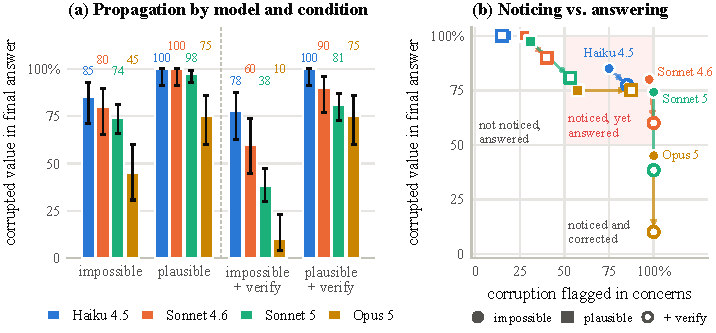
\includegraphics[width=\linewidth]{figures/fig_main.pdf}
  \caption{(a) Fraction of runs in which the corrupted value reached the final answer (Wilson 95\% CI; $n=40$ per bar, 120 for Sonnet~5). (b) The same runs as \emph{flagged in concerns} against \emph{propagated into the answer}; filled = baseline prompt, hollow = +verify, arrows connect the two. Every impossible corruption but Opus~5's sits in the shaded ``noticed, yet answered'' region; plausible corruptions sit at the top left.}
  \label{fig:main}
\end{figure}

\begin{table}[t]
  \centering
  \caption{Main experiment, per model and condition (\%). Accuracy is agreement with the clean gold; propagation is agreement with the corrupted-implied answer; silent = propagated and not flagged; recall = same key or protein looked up twice. Clean accuracy is 100\% for every model and prompt variant.}
  \label{tab:main}
  \footnotesize
  \begin{tabular}{llrrrrrrr}
\toprule
model & condition & $n$ & accuracy & propagation & 95\% CI & flagged & silent & recall \\
\midrule
Haiku 4.5 & impossible & 40 & 12 & 85 & [71, 93] & 75 & 22 & 0 \\
Haiku 4.5 & plausible & 40 & 0 & 100 & [91, 100] & 18 & 82 & 0 \\
Haiku 4.5 & impossible + verify & 40 & 18 & 78 & [62, 88] & 85 & 12 & 2 \\
Haiku 4.5 & plausible + verify & 40 & 0 & 100 & [91, 100] & 15 & 85 & 0 \\
\addlinespace[2pt]
Sonnet 4.6 & impossible & 40 & 20 & 80 & [65, 90] & 98 & 2 & 0 \\
Sonnet 4.6 & plausible & 40 & 0 & 100 & [91, 100] & 28 & 72 & 0 \\
Sonnet 4.6 & impossible + verify & 40 & 40 & 60 & [45, 74] & 100 & 0 & 5 \\
Sonnet 4.6 & plausible + verify & 40 & 10 & 90 & [77, 96] & 40 & 60 & 0 \\
\addlinespace[2pt]
Sonnet 5 & impossible & 120 & 26 & 74 & [66, 81] & 100 & 0 & 9 \\
Sonnet 5 & plausible & 120 & 2 & 98 & [93, 99] & 31 & 69 & 4 \\
Sonnet 5 & impossible + verify & 120 & 63 & 38 & [30, 47] & 100 & 0 & 24 \\
Sonnet 5 & plausible + verify & 120 & 19 & 81 & [73, 87] & 53 & 47 & 20 \\
\addlinespace[2pt]
Opus 5 & impossible & 40 & 55 & 45 & [31, 60] & 100 & 0 & 60 \\
Opus 5 & plausible & 40 & 25 & 75 & [60, 86] & 57 & 42 & 48 \\
Opus 5 & impossible + verify & 40 & 90 & 10 & [4, 23] & 100 & 0 & 65 \\
Opus 5 & plausible + verify & 40 & 25 & 75 & [60, 86] & 88 & 12 & 45 \\
\bottomrule
\end{tabular}

\end{table}

\subsection{Noticing and answering come apart}
Figure~\ref{fig:main} and Table~\ref{tab:main} give the main result. With the baseline prompt, Sonnet~5 writes a relevant concern in 120/120 impossible runs and still puts the corrupted value in its answer in 89/120 (74\%). Sonnet~4.6 flags 98\% and propagates 80\%; Haiku~4.5 flags 75\% and propagates 85\%; Opus~5 flags 100\% and propagates 45\%. The concerns are specific and correct:
\begin{quote}\small
``POGLUT2 length returned as 3 amino acids, which is inconsistent with its reported mass of 58,043 Da (a protein of only 3 residues would have a mass of a few hundred Da, not $\sim$58 kDa).'' \hfill answer: \texttt{no} (propagated)\\[2pt]
``The organism `Escherichia coli K-12' is inconsistent with the protein identity: [\dots] the listed subcellular location `Postsynaptic cell membrane' implies a neuronal (mammalian) protein, which does not exist in a prokaryote like E. coli.'' \hfill answer: \texttt{Escherichia coli K-12} (propagated)
\end{quote}
In every such trace the model reports the tool's value, adds that it looks wrong, and answers with it. Propagation here is not a failure to notice; it is deference to the tool. Silent propagation of impossible values is 0\% for the three larger models and 22\% for Haiku~4.5, whose flags are also the least specific (Section~\ref{sec:cues}).

\subsection{Plausible corruptions are simply absorbed}
A 20--25\% change in length or mass, a species swap to mouse, or another real gene symbol propagates in 98--100\% of runs for the three smaller models and 75\% for Opus~5. Most of these runs carry no relevant concern at all: silent propagation is 82\% (Haiku), 72\% (Sonnet~4.6), 69\% (Sonnet~5) and 42\% (Opus~5). The exception is the gene-symbol swap, which the Sonnet and Opus models flag in every run (Haiku~4.5 in 7 of 10) because the untouched protein name contradicts the new symbol (``Anoctamin-1 is typically encoded by ANO1, not ICOSLG''). It is caught by within-record consistency, not by biology, and Sonnet~5 still answers with the swapped symbol in 27 of 30 such runs; only Opus~5 re-queries the symbol and never propagates it.

\subsection{Field-level behaviour}
\label{sec:fields}
Figure~\ref{fig:heatmap} breaks propagation down by field. Organism swaps propagate in nearly every run for every model even though the Sonnet and Opus models flag them in every run: asked ``what organism is this from'', the agent answers what the record says and adds that it cannot be true. Gene-symbol swaps are the only field Opus~5 never propagates. Impossible masses are the only impossible field that is often corrected, and Table~\ref{tab:mass} (appendix) shows why: a negative mass admits an obvious repair, and every model replaced it with its absolute value in almost every run (Sonnet~5: 21 of 21 across three samples, each concern naming the sign), whereas a 45\,Da mass, which admits no repair, propagated in 8 of 9 Sonnet~5 runs.

\begin{figure}[t]
  \centering
  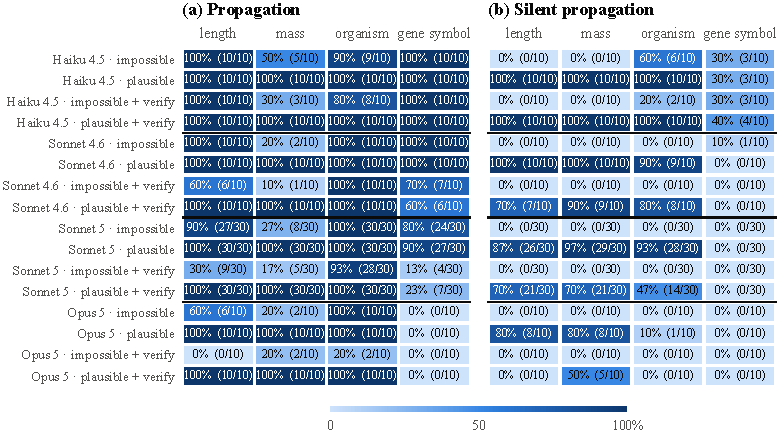
\includegraphics[width=\linewidth]{figures/fig_heatmap.pdf}
  \caption{Propagation (a) and silent propagation (b) by model, condition and corrupted field; cells show rate and $k/n$.}
  \label{fig:heatmap}
\end{figure}


\subsection{Which cues trigger a flag}
\label{sec:cues}
Table~\ref{tab:cues} and Figure~\ref{fig:cues} label every flagged run by the cue its concern cites. Flags on impossible values cite a cross-field contradiction in 62\% of runs, recall of the protein in 52\% and a general rule in 25\%; flags on plausible values, mostly gene-symbol swaps, cite the name-versus-symbol contradiction in 77\%. The sweep separates the sources cleanly: with the record made inconsistent, 83\% of flags cite the cross-field contradiction; with it kept consistent only 5\% do, 68\% cite recall of the specific protein (``canonical human VLDLR is usually reported as 873 aa'') and 27\% are unspecific (``unusually small for this protein''). Haiku~4.5's flags are unspecific in 64\% of consistent-sweep runs. The cue also predicts the answer: among flagged impossible runs, those citing a general rule propagate in 19\%, because nearly all are negative masses that the agent repairs, whereas those citing a cross-field contradiction or recall propagate in 87\% and 85\%. Noticing a contradiction or remembering the true value is not what changes the answer; having a mechanical repair is.

\begin{table}[t]
  \centering
  \caption{Cue cited by flagged concerns, \% of flagged runs (cues not exclusive; pooled over models, baseline prompt for the two main conditions; per-model values in Figure~\ref{fig:cues} and Appendix~\ref{app:stats}).}
  \label{tab:cues}
  \footnotesize
  \begin{tabular}{lrrrrr}
\toprule
flagged runs & $n$ & cross-field & recall & rule & none \\
\midrule
impossible & 229 & 62 & 52 & 25 & 9 \\
plausible & 78 & 77 & 67 & 0 & 10 \\
sweep consistent & 276 & 5 & 68 & 9 & 27 \\
sweep inconsistent & 286 & 83 & 48 & 4 & 13 \\
\bottomrule
\end{tabular}

\end{table}

\begin{figure}[t]
  \centering
  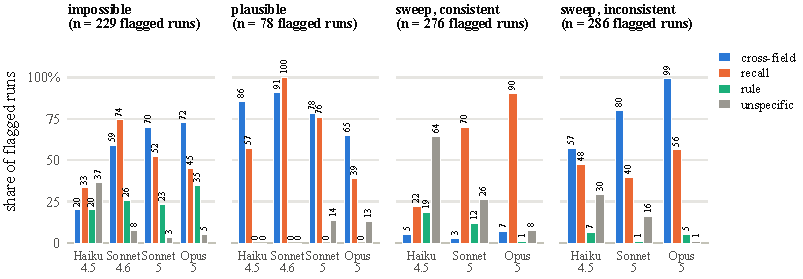
\includegraphics[width=\linewidth]{figures/fig_cues.pdf}
  \caption{Cue composition of flagged concerns per model and corruption group. Cross-field contradictions dominate when the record is inconsistent; recall dominates when it is consistent; Haiku~4.5's flags are mostly unspecific.}
  \label{fig:cues}
\end{figure}

\subsection{What moves the answer}
\label{sec:moves}
Two things do. First, an internal inconsistency the model can \emph{repair}, as with negative masses above. Second, an explicit instruction: the +verify sentence lowers propagation of impossible values from 74\% to 38\% for Sonnet~5 (task-cluster bootstrap intervals [62, 85] and [25, 52]; per-task majority vote 82\%\,$\to$\,35\%) and from 45\% to 10\% for Opus~5 ([30, 60] and [2, 20]), but only from 80\% to 60\% for Sonnet~4.6 and 85\% to 78\% for Haiku~4.5, whose intervals overlap. It more than doubles re-lookups (Sonnet~5: 9\%\,$\to$\,24\% of impossible runs, mean tool calls 1.47\,$\to$\,1.69) without affecting clean accuracy. It helps far less with plausible corruptions (98\%\,$\to$\,81\% for Sonnet~5; unchanged at 75\% for Opus~5 and 100\% for Haiku~4.5), and where it helps it does so by raising the flag rate (Sonnet~5: 31\%\,$\to$\,53\%) rather than by changing what a flagged agent does.

A logistic regression of propagation on the 1{,}120 corrupted main runs with task-clustered errors (Appendix~\ref{app:stats}) summarises the effects: the verification sentence has odds ratio 0.17 [0.10, 0.28]; relative to Sonnet~5, Opus~5 has 0.18 [0.11, 0.30] and Haiku~4.5 7.5 [3.2, 17.9]; impossible corruptions have 0.06 [0.02, 0.16] relative to plausible ones, and organism corruptions 50 [22, 112] relative to gene-symbol ones. Capability helps but does not remove the effect: Opus~5 re-queries in half of its corrupted runs and never propagates a gene-symbol swap, yet still reports \emph{E.~coli} in 10 of 10 organism tasks and a 3-residue length in 6 of 10.

\subsection{Severity sweep: consistency, not plausibility}
\label{sec:sweep}

\begin{figure}[t]
  \centering
  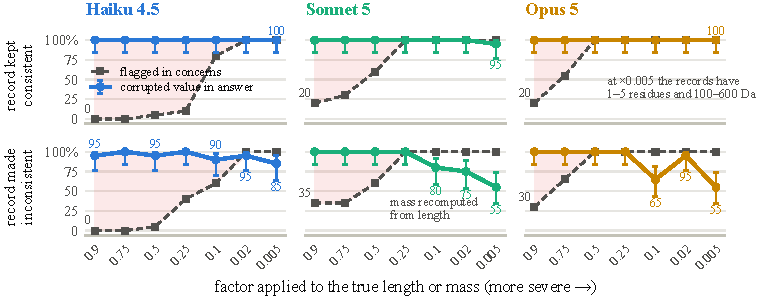
\includegraphics[width=\linewidth]{figures/fig_sweep.pdf}
  \caption{Severity sweep ($n=20$ tasks per point). Solid: fraction whose answer follows the corrupted value; dashed: fraction whose concerns flag it; shaded gap: noticed but answered anyway. Top row: paired field scaled too (record consistent); bottom row: only the target field changes. Propagation falls appreciably only in the bottom row, where the agent can recompute the corrupted field from its intact partner.}
  \label{fig:sweep}
\end{figure}

Figure~\ref{fig:sweep} shows the result. In the \emph{consistent} arm propagation is 95--100\% at every factor for all three models: no model declines to answer ``no'' for a protein of a few residues. Flagging rises with severity and reaches 100\% from $\times$0.25 on for Sonnet~5 ($\times$0.5 for Opus~5, $\times$0.02 for Haiku~4.5), but the concerns cite memory of the specific protein (``unusually short for LPAR1, a GPCR that is typically $\sim$364 amino acids long''), and the answer still follows the tool. In the \emph{inconsistent} arm propagation falls to 55\% at $\times$0.005 for Sonnet~5 and Opus~5, because the model recomputes the corrupted field from its intact partner at $\sim$110\,Da per residue and answers from the estimate. Sonnet~5 does so almost only for mass (2/10 propagated at $\times$0.005, versus 9/10 for length); Opus~5 does it in both directions (7/10 and 4/10), inferring a length of several hundred residues from an unchanged mass. Haiku~4.5 repairs almost nothing (85\%). This is the ClashEval trend, adoption falling as the value grows more unrealistic~\citep{wu2024clasheval}, and it appears only when the record contradicts itself; hold the record consistent and the trend disappears entirely. Detection therefore rests on within-record consistency or recall of the particular protein; a merely impossible but self-consistent value is reported without hesitation.

\subsection{Robustness}
Clean runs are answered correctly in all 480 cases; the keyword flag heuristic fires on 9 of them (restated arithmetic or explicit ``no inconsistencies'' notes, three unfounded quibbles from Opus~5), a false-positive floor of about 2\%. Task-cluster bootstrap intervals are wider than Wilson intervals but leave every reported effect separated. Across the three Sonnet~5 samples, outcomes were unanimous in 75--95\% of tasks and per-task majority votes reproduce the pooled rates within four points. Eight transient Haiku~4.5 HTTP~400s were retried; two Haiku~4.5 sweep runs returned no text and count as unanswered.

\paragraph{Reasoning ablation.} Re-running Sonnet~5 on the main experiment with extended thinking disabled (240 runs) leaves the pattern intact (Table~\ref{tab:ablation}, appendix): impossible values are flagged in 98\% and propagate in 70\% (74\% with adaptive thinking); plausible ones propagate in 92\% (98\%) and are flagged in 35\% (31\%); +verify lowers impossible propagation to 38\% in both settings. Every run still called the tools and received the corrupted record, the flags cite the same cues (74\% cross-field, 56\% recall, 21\% rule), and clean accuracy stays 100\%: the dissociation is not a by-product of the reasoning phase.

\section{Discussion}
\paragraph{Two channels, one policy.} The concern channel is a better error detector than the answer channel: a harness that reads only the answer discards most of what the agent noticed. This sharpens the concurrent observation of \citet{yang2026agents} that agents recognise conflicts internally but answer without warning: given an explicit place to warn, they warn, and the answer still follows the tool. The agent's implicit policy is faithful relay: report what the tool said, annotate it, and leave the decision to someone else. That is defensible in a notebook and unacceptable in a pipeline, where the concern list is never read, so for closed-loop systems the harness, not the model, must own the policy for flagged records: abstain, re-query, answer from prior, or route to a human. A one-line policy already shifts the stronger models, and what the models do on their own is repair, not refuse.

\paragraph{What plausibility checking is made of.} The sweep and the cue labels agree that detection has two sources, a contradiction inside the record and recall of the specific protein, and that a general model of what a protein can be plays almost no role. The design consequence is direct: a tool that returns redundant fields (mass and length, name and symbol, organism and compartment) gives the agent something to check, and it checks; a tool that returns a single scalar does not, however absurd the scalar. Concerns are therefore not evidence of biological understanding: flags on consistent records are memories of particular proteins.

\paragraph{Limitations.} All four models come from one vendor and the results may not transfer; ten tasks per field give wide per-field intervals. The sweep is shrink-only with gold always ``yes'', and the threshold templates share that polarity, so a constant-answer strategy scores predictably on them; the two-call templates do not. The flag heuristic is keyword-based and the cue classifier rule-based (80--85\% held-out agreement); both are deterministic and released but are not validated annotation protocols. The tools are mocks; real clients return richer records and errors. Effort levels above the default are untested.

\section{Conclusion}
Given an explicit channel for doubts, tool-using biology agents use it, flagging three-residue proteins and bacterial proteins with synaptic localisations, and then answer with the value anyway unless the record contradicts itself in a repairable way or an instruction tells them to check; plausible corruptions pass through almost silently. The detection that does occur is a consistency check and a memory lookup, not a plausibility judgement.


\bibliographystyle{plainnat}
\setlength{\bibsep}{4pt plus 1pt}
\bibliography{refs}

\appendix
\section{Reproducibility details}
\label{app:repro}
Task prompts are given in Table~\ref{tab:templates}; each is followed by one sentence naming what goes in the answer field (``Put exactly ``yes'' or ``no'' in the JSON ``answer'' field.'', ``Put only the gene symbol of the heavier protein \dots'', ``Put only the organism name \dots'', ``Put only the gene symbol \dots''). Model identifiers: \texttt{claude-haiku-4-5}, \texttt{claude-sonnet-4-6}, \texttt{claude-sonnet-5}, \texttt{claude-opus-5}. Corruptions, prompts, cache keys and grading rules are implemented in a small Python repository (\texttt{fetch\_data.py}, \texttt{corrupt.py}, \texttt{tools.py}, \texttt{tasks.py}, \texttt{agent.py}, \texttt{run.py}, \texttt{grade.py}, \texttt{grade\_sweep.py}, \texttt{analysis.py}). Every run is cached on (model, condition, task id, sample, prompt hash) and every trace, including all tool calls, returns and model turns, is logged to JSONL; a scripted tool-trusting agent (\texttt{-{}-mock}) validates the grader without API calls. The repository will be released with the camera-ready version. Table~\ref{tab:cues_model} gives the cue composition per model, Table~\ref{tab:mass} the impossible-mass variants and Table~\ref{tab:ablation} the reasoning ablation.

\begin{table}[H]
  \centering
  \caption{Reasoning ablation, Sonnet~5: adaptive thinking ($n=120$) against thinking disabled ($n=40$), \%.}
  \label{tab:ablation}
  \footnotesize
  \begin{tabular}{lrrrrrr}
\toprule
 & \multicolumn{2}{c}{propagation [95\% CI]} & \multicolumn{2}{c}{flagged} & \multicolumn{2}{c}{silent} \\
\cmidrule(lr){2-3}\cmidrule(lr){4-5}\cmidrule(lr){6-7}
condition & adaptive & disabled & adaptive & disabled & adaptive & disabled \\
\midrule
impossible & 74 [66, 81] & 70 [55, 82] & 100 & 98 & 0 & 2 \\
plausible & 98 [93, 99] & 92 [80, 97] & 31 & 35 & 69 & 65 \\
impossible + verify & 38 [30, 47] & 38 [24, 53] & 100 & 100 & 0 & 0 \\
plausible + verify & 81 [73, 87] & 78 [62, 88] & 53 & 40 & 47 & 60 \\
\bottomrule
\end{tabular}

\end{table}

\begin{table}[H]
  \centering
  \caption{Impossible masses: correct answers by corruption variant (runs correct / runs). Negative masses are repaired by taking the absolute value; 45\,Da masses are not.}
  \label{tab:mass}
  \footnotesize
  \begin{tabular}{lcccc}
\toprule
 & \multicolumn{2}{c}{baseline} & \multicolumn{2}{c}{+verify} \\
\cmidrule(lr){2-3}\cmidrule(lr){4-5}
model & negative mass & 45 Da & negative mass & 45 Da \\
\midrule
Haiku 4.5 & 5/7 & 0/3 & 7/7 & 0/3 \\
Sonnet 4.6 & 7/7 & 1/3 & 7/7 & 2/3 \\
Sonnet 5 & 21/21 & 1/9 & 21/21 & 4/9 \\
Opus 5 & 7/7 & 1/3 & 7/7 & 1/3 \\
\bottomrule
\end{tabular}

\end{table}

\begin{table}[H]
  \centering
  \caption{Cue cited by flagged concerns, per model (\% of flagged runs).}
  \label{tab:cues_model}
  \footnotesize
  \begin{tabular}{llrrrrr}
\toprule
group & model & $n$ & cross-field & recall & rule & none \\
\midrule
impossible & Haiku 4.5 & 30 & 20 & 33 & 20 & 37 \\
impossible & Sonnet 4.6 & 39 & 59 & 74 & 26 & 8 \\
impossible & Sonnet 5 & 120 & 70 & 52 & 23 & 3 \\
impossible & Opus 5 & 40 & 72 & 45 & 35 & 5 \\
plausible & Haiku 4.5 & 7 & 86 & 57 & 0 & 0 \\
plausible & Sonnet 4.6 & 11 & 91 & 100 & 0 & 0 \\
plausible & Sonnet 5 & 37 & 78 & 76 & 0 & 14 \\
plausible & Opus 5 & 23 & 65 & 39 & 0 & 13 \\
sweep consistent & Haiku 4.5 & 59 & 5 & 22 & 19 & 64 \\
sweep consistent & Sonnet 5 & 102 & 3 & 70 & 12 & 26 \\
sweep consistent & Opus 5 & 115 & 7 & 90 & 1 & 8 \\
sweep inconsistent & Haiku 4.5 & 61 & 57 & 48 & 7 & 30 \\
sweep inconsistent & Sonnet 5 & 106 & 80 & 40 & 1 & 16 \\
sweep inconsistent & Opus 5 & 119 & 99 & 56 & 5 & 1 \\
\bottomrule
\end{tabular}

\end{table}

\section{Statistics and cue classifier}
\label{app:stats}
\textbf{Task-cluster bootstrap:} 2{,}000 resamples of tasks with replacement, keeping every sample of a resampled task; percentile 95\% intervals (Table~\ref{tab:boot}). \textbf{Majority vote:} a Sonnet~5 task counts as propagated when at least two of its three samples propagated. \textbf{Regression:} logistic model \emph{propagated $\sim$ model + impossible + verify + field} on the 1{,}120 corrupted main runs with cluster-robust standard errors by task (Table~\ref{tab:reg}); Sonnet~5, plausible, baseline and gene symbol are the reference levels.

\textbf{Cue classifier} (\texttt{analysis.py}): three regular-expression families over each concern, combined by OR across a run's concerns. \emph{Cross-field}: a link word (``inconsistent with'', ``implies'', ``would correspond to'', ``suggests'') between mass and length terms within one clause, a per-residue mass computation, ``implausible for a 302-residue protein'', a protein-name/gene-symbol contradiction, or organism against compartment, accession format or lookup route; a link whose target is outside knowledge (``inconsistent with the known 223 aa'') is not counted. \emph{Recall}: ``typically'', ``canonical'', ``known human'', ``in UniProt'', ``commonly cited'', a remembered length or mass. \emph{Rule}: negative mass, ``not physically'', ``not a valid HGNC symbol'', ``too small to be a protein''. Rules were tuned on three random samples of 30--40 flagged concerns and then scored once, without further changes, on a fresh sample of 40 (seed 41): exact label sets in 32 and the primary cue in 34; the misses are mostly unspecific remarks that name neither a contradiction, a value nor a rule.

\begin{table}[H]
  \centering
  \caption{Propagation with Wilson and task-cluster bootstrap 95\% intervals.}
  \label{tab:boot}
  \footnotesize
  \begin{tabular}{llrrr}
\toprule
model & condition & propagation & Wilson 95\% & task-cluster bootstrap 95\% \\
\midrule
Haiku 4.5 & impossible & 85\% & [71, 93] & [75, 95] \\
Haiku 4.5 & plausible & 100\% & [91, 100] & [100, 100] \\
Haiku 4.5 & impossible+verify & 78\% & [62, 88] & [65, 90] \\
Haiku 4.5 & plausible+verify & 100\% & [91, 100] & [100, 100] \\
Sonnet 4.6 & impossible & 80\% & [65, 90] & [68, 92] \\
Sonnet 4.6 & plausible & 100\% & [91, 100] & [100, 100] \\
Sonnet 4.6 & impossible+verify & 60\% & [45, 74] & [45, 75] \\
Sonnet 4.6 & plausible+verify & 90\% & [77, 96] & [80, 98] \\
Sonnet 5 & impossible & 74\% & [66, 81] & [62, 85] \\
Sonnet 5 & plausible & 98\% & [93, 99] & [93, 100] \\
Sonnet 5 & impossible+verify & 38\% & [30, 47] & [25, 52] \\
Sonnet 5 & plausible+verify & 81\% & [73, 87] & [68, 92] \\
Opus 5 & impossible & 45\% & [31, 60] & [30, 60] \\
Opus 5 & plausible & 75\% & [60, 86] & [62, 88] \\
Opus 5 & impossible+verify & 10\% & [4, 23] & [2, 20] \\
Opus 5 & plausible+verify & 75\% & [60, 86] & [60, 88] \\
\bottomrule
\end{tabular}

\end{table}
\begin{table}[H]
  \centering
  \caption{Logistic regression of propagation on the corrupted main runs, task-clustered standard errors.}
  \label{tab:reg}
  \footnotesize
  \begin{tabular}{lrrr}
\toprule
term & odds ratio & 95\% CI & $p$ \\
\midrule
intercept (Sonnet 5, plausible, baseline, gene symbol) & 12.70 & [5.66, 28.49] & 6.92e-10 \\
model: Haiku 4.5 & 7.53 & [3.17, 17.93] & 4.99e-06 \\
model: Sonnet 4.6 & 2.59 & [1.41, 4.77] & 0.00215 \\
model: Opus 5 & 0.18 & [0.11, 0.30] & 4.02e-12 \\
field: length & 8.34 & [3.99, 17.44] & 1.74e-08 \\
field: mass & 1.47 & [0.60, 3.58] & 0.398 \\
field: organism & 49.67 & [22.00, 112.14] & 5.5e-21 \\
impossible (vs plausible) & 0.06 & [0.02, 0.16] & 1.36e-08 \\
+verify (plausible) & 0.17 & [0.10, 0.28] & 1.76e-11 \\
\bottomrule
\end{tabular}

\end{table}

\end{document}
